\begin{figure}[H]
    \centering
    \begin{adjustbox}{width=12cm,center}
    \frame{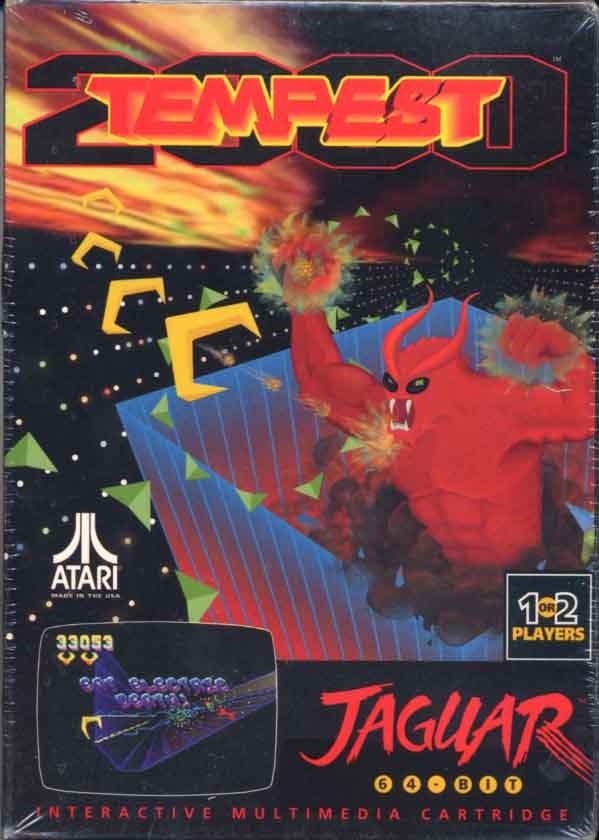
\includegraphics{src/preface/tempest.png}}%
    \end{adjustbox}
\caption{Cover art for Tempest 2000}
\end{figure}
\clearpage
\chapter*{about this book} 
Tempest 2000 was a classic game. To its misfortune it was made for a console that crashed and burned with no
survivors. The Atari Jaguar was supposed to be gaming's first great leap into the 64 bit era. Instead it 
promptly tripped over its shoelaces and left a number of great games, Tempest 2000 among them, behind
as orphans.

This is a book about computer code. Each chapter aims to be an easily digested sketch of how
a specific feature or effect was achieved using a combination of Motorola 68K assembly code and
the Jaguar's powerful hardware platform.

There are lots of fascinating bits and pieces to pore over. These are the 25 easiest I could find.

%\begin{figure}[H]
%    \begin{adjustbox}{width=10cm,center}
%    \frame{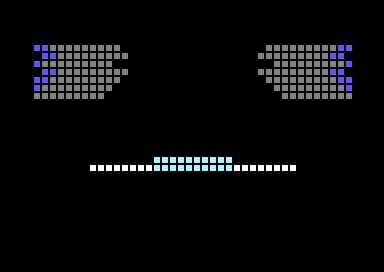
\includegraphics{src/preface/p1.png}}%
%      \hspace{0.1cm}
%    \frame{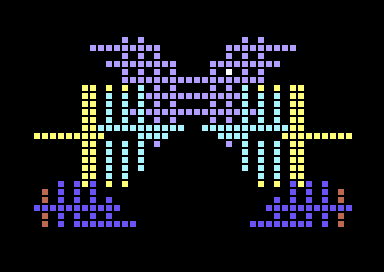
\includegraphics{src/preface/p2.png}}%
%    \end{adjustbox}
%\end{figure}
%\vspace{-0.8cm}
%\begin{figure}[H]
%    \begin{adjustbox}{width=10cm,center}
%    \frame{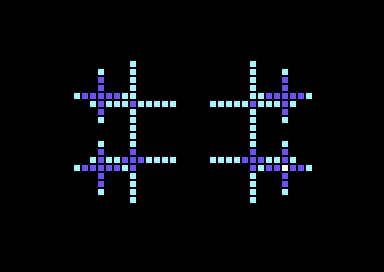
\includegraphics{src/preface/p3.png}}%
%      \hspace{0.1cm}
%    \frame{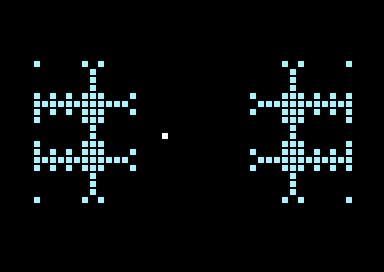
\includegraphics{src/preface/p4.png}}%
%    \end{adjustbox}
%\end{figure}

Rob Hogan (\href{https://mastodon.social/@mwenge}{\textcolor{blue}{@mwenge}})\\
Dublin \the\year{} \\

\clearpage
\vspace*{\fill}
\begin{figure}[H]
    \centering
      
\includegraphics[width=5cm]{src/cover/title_page.png}%
\end{figure}
\vspace*{\fill}
\thispagestyle{empty}%
\clearpage

